\chapter{INSERT}
\label{LitRev}
% general system design
% Detection module 
% collimator
% Hardware evaluation/ PSMR paper 
% Current state (Milan experiments and London installation)
% Calibration procedure
% Software Pera and Bulma % software (PERA pg 137 Deb. 65 Il.)

\section{Introduction and Motivations}
As discussed in the last chapter the development of a \acrshort{SPECT/MRI} will provide many advantages due to the diverse applications that the individual \acrshort{SPECT} and \acrshort{MRI} systems have \cite{doi:10.1259/bjr.20160690}. Combined \acrshort{SPECT/MRI} data can be used to determine functional information from brain scans of known tumours in order to track development and plan treatments. The advantage of introducing \acrshort{MR} into nuclear imaging system is that of an improved soft tissue imaging and reduce dose, compared to that of \acrshort{CT}. The range of \acrshort{MR} protocols such as functional \acrshort{MR} also promises many advantages over \acrshort{SPECT/CT}. However \acrshort{SPECT} and \acrshort{PET} are not easily integrated into the \acrshort{MR} environment. 
\paragraph{}
The strong magnetic fields produced by the \acrshort{MRI} introduce electromagnetic interference between the devices. Technology such as \acrshort{PMT} cannot function within a strong magnetic field and the presences of external electromagnetic signals will deter the imaging capabilities of the \acrshort{MR}. These challenges have been overcome in \acrshort{PET/MR} with the development of solid state light detectors which are capable of functioning within a magnetic field.

Although the use of \acrshort{SPECT} can provide advantages in \acrshort{MR} \cite{doi:10.1177/153303460600500406}, it introduces further compatibility issues. \acrshort{SPECT} is typically a dynamic system, in which a moving camera head will acquire data. This is not possible within \acrshort{MRI}; as well as the physical space required by a moving gantry, the reactive forces generated by the motor can damage the gradient coils within the \acrshort{MR}. A stationary system must be adapted and so sampling angles are sacrificed. The second consideration is the presence of the collimator. These are typically made of a lead alloy which is ferrous. In order to function within the \acrshort{MR}, the collimator must be redesigned to include non-ferrous elements. 
\paragraph{}
The challenges encountered when combine \acrshort{SPECT} with \acrshort{MR} were tackled in the development of the \acrshort{INSERT} scanner. The \acrshort{INSERT} project aims to develop the worlds first clinical \acrshort{SPECT} insert capable of simultaneous use within a \acrshort{MRI} system. The project sets out to achieve this goal in order to provide a tool for the stratification of glioma tumour therapy. In establishing this novel technology the project can lay the ground work for completely integrated \acrshort{SPECT/MRI} systems.

\section{INSERT Project}
In order to establish an \acrshort{MR} compatible \acrshort{SPECT}, \acrshort{INSERT} implemented a set of unique design features. The system is composed of a partial ring of 20 stationary detector units. This minimises the dimensions and allows it to fit within the bore of a clinical \acrshort{MRI}. Each detector head is composed of a \acrlong{CsITl} (\acrshort{CsITl}) crystal, \acrlong{SiPM} (\acrshort{SiPM}) and \acrlong{ASIC} (\acrshort{ASIC}) readout \cite{Trigilio2018AApplications}. The \acrshort{MR} compatible technology was proven in \acrshort{PET/MR} systems and had been specially designed for the \acrshort{INSERT}. A novel \acrshort{MR} compatible collimator composed of tungsten was developed; the \acrlong{MSS} (\acrshort{MSS}) \cite{7430894}. Together these components produced a compact stand alone \acrshort{SPECT} scanner. In order to use this within an \acrshort{MR} a \acrlong{RF} coil is required. This is a standard component in \acrshort{MRI} systems, however, in order to work within the \acrshort{INSERT}, it is essential that the coil fits within the bore of the \acrshort{INSERT} and can transmit and receive the \acrshort{RF} pulses. The \acrshort{RF} pulses must be transmitted from within the \acrshort{INSERT} bore so the pulse signal does not travel through the \acrshort{INSERT}, as this could damage the detector electronics and collapse the \acrshort{MR} signal.
\paragraph{}
One of this thesis' goals is the evaluation of the stand alone \acrshort{SPECT} system. Upon completion of the \acrshort{INSERT} scanner, it has undergone extensive electrical and stability testing \cite{8432104}, however the imaging capability of the novel system has yet to be established. The system components are outlined here in order to establish the current state of the \acrshort{INSERT} (figure \ref{fig:INSERT}).

\begin{figure}[!tbp]
  \centering
  \subfloat[The INSERT scanner.]{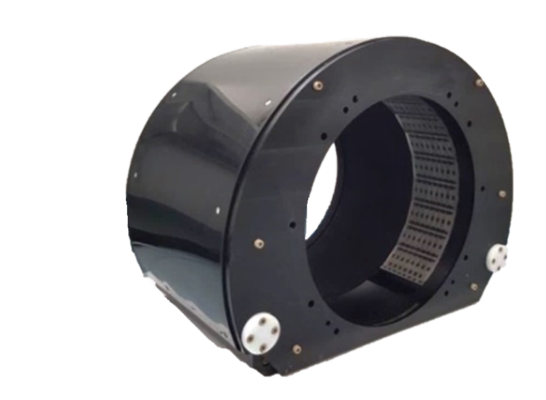
\includegraphics[width=0.5\textwidth]{figures/INSERT_covered.png}\label{fig:INSERT}}
  \hfill
  \subfloat[The INSERT design without its cover.]{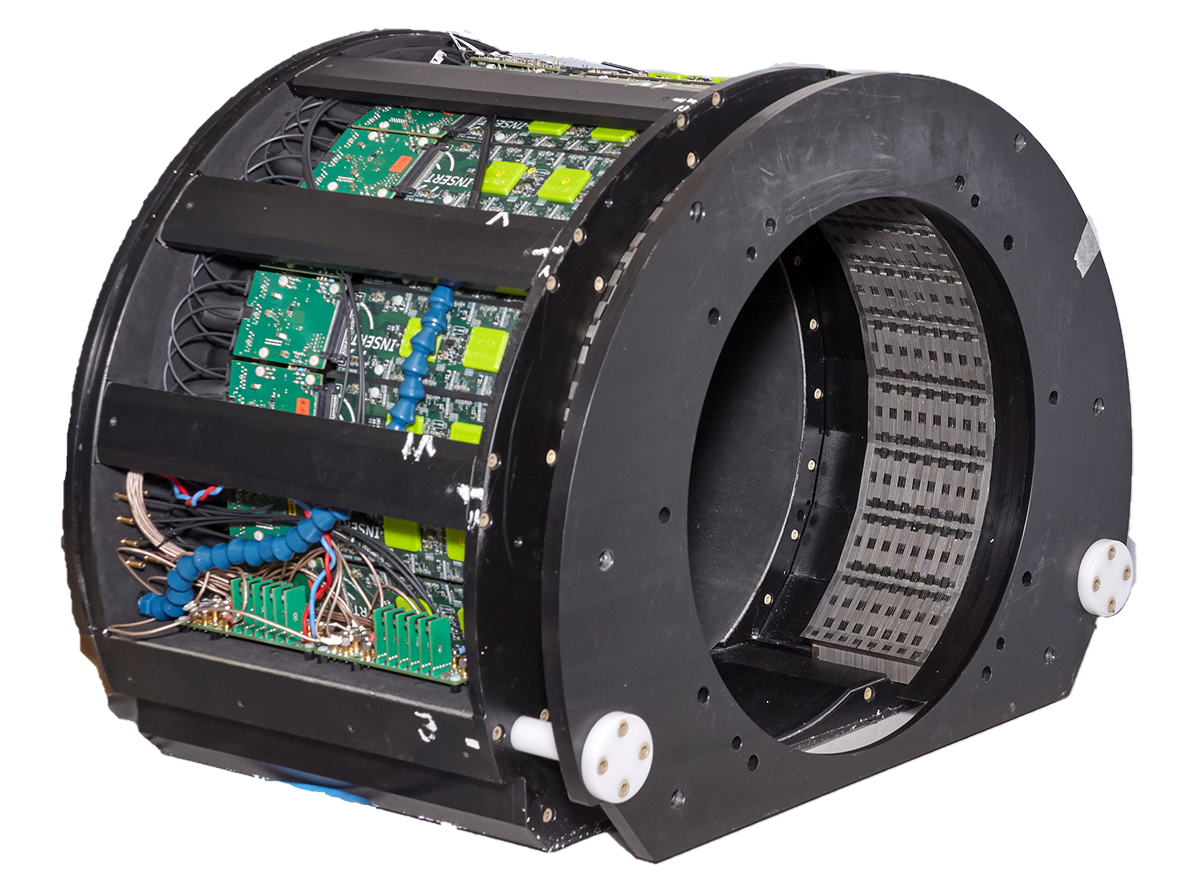
\includegraphics[width=0.5\textwidth]{figures/INSERT_foto1.png}\label{fig:INSERT2}}
  \caption{This tabletop SPECT scanner is composed of 20 detector heads which come together in a compact stationary system.}
\end{figure}

\subsection{Detector Units}
The first components we consider are the 20 gamma detector heads.  The devices chosen in the INSERT design are a \acrshort{CsITl} crystal coupled to a \acrshort{SiPM} (figure \ref{fig:DetUnit}) \cite{7430864} \cite{Occhipinti2016AApplications}. The \acrshort{CsITl} crystal covered 100 mm x 50 mm with a 8 mm thickness. The crystal thickness imposes a compromise between absorption and spatial resolution. \acrshort{CdTe} crystal have also proven successfully \cite{Cai2010ADetectors} however they did provide the same performance for a compact design compared to the \acrshort{CsITl}. The crystal dimensions were chosen to maintain a compact system; \acrshort{CsITl} provided a greater spatial resolution and efficiency, which is essential in the detection of low energy gamma rays.

\begin{figure}[!t]
%\vspace{-0.2cm}
\centering
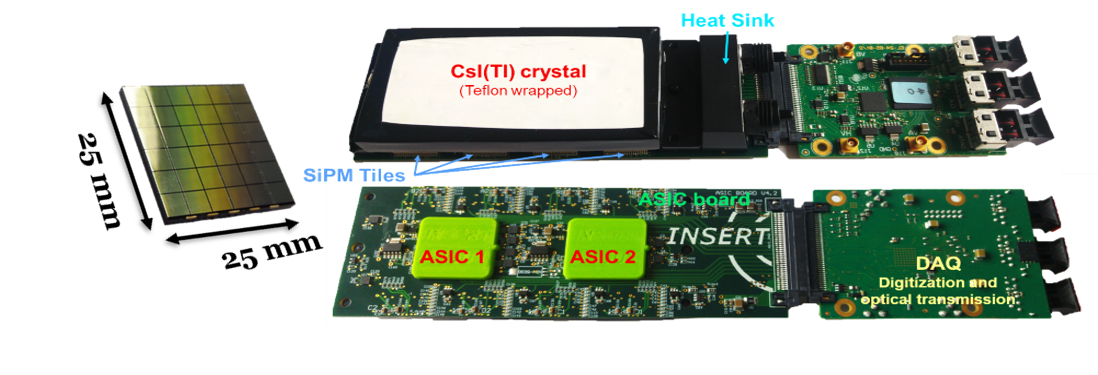
\includegraphics[width=5in]{figures/detector.png}

    \caption{The detector units used in the \acrshort{INSERT} including the heat sink for cooling. Each \acrshort{SiPM} tile is composed of a 25x25 mm macrocell.} \label{fig:DetUnit}
%\vspace{-0.2cm}
\end{figure}

\paragraph{}
\acrshort{SiPM} have proven successful in \acrshort{PET/MR} systems and have shown promising results within the \acrshort{MR} environment \cite{MCELROY2007106}. Many scanners implement \acrshort{APD} detectors, however, \acrshort{SiPM} have a greater gain, time resolution and sensitivity \cite{RENKER200648} \cite{Wagatsuma2017ComparisonTOF-PET/CT}.  \acrshort{SiPM} was chosen as it is a compact solid state device able to function within a strong magnetic field \cite{SCHAART201631} \cite{0031-9155-56-23-014} \cite{DINU2015367}. A \acrshort{SiPM} is composed in a microcell, a series of \acrshort{SiPM} arranged together each generating a combined \acrshort{G-APD} avalanche signal \cite{DINU2015367}. The \acrshort{SiPM} are arranged in a minimally spaced array to cover the detector surface with maximum light detection. \acrshort{SiPM} are susceptible to \acrlong{DCR}; this is a false signal caused by the production of electron positron pairs. \acrshort{DCR} is prominent during operation with lower energy nuclides in \acrshort{SPECT}. The \acrshort{DCR} is related to the thermal response of the detector and so the \acrshort{SiPM} requires a cooling unit to maintain a functioning temperature. The detector design was initialised in the preclinical system \cite{7287793}.
\paragraph{}
The detector makes use of 72 channels (\acrshort{SiPM} macrocells) for ease of processing. The data collected from the detector heads are processed with the methods described in chapter \ref{Introduction}. The \acrshort{ML} algorithm is implemented in two software used throughout this body of work; \acrshort{PERA} (\acrlong{PERA}) \cite{OCCHIPINTI2015DevelopmentImaging}, and INSERT GUI software provided by Mediso Ltd. As discussed the \acrshort{ML} requires a model to carry out the optimisation, the algorithm used in \acrshort{PERA} makes use of an initial centroid reconstruction and a series of \acrshort{SiPM} models known as \acrlong{LRF}s. The \acrshort{LRF} is the average response of each individual channel as a function of the event position; this maps each event position within the crystal to each given photodetector. These models are calculated by building an iterative model from experimental data \cite{Morozov_2017} \cite{8069405}. The \acrshort{LRF} are created once from a flood acquisition and can be used in all subsequent reconstructions. The reconstruction carried out by the \acrshort{INSERT} system follows several steps. An energy window is defined about the photopeak and events which do not fall within the window are removed. Coordinates (X,Y) in projection space are initialised with a \textbf{modified centroid}. The coordinates are optimised in the \acrshort{ML} by using the \acrshort{LRF} models: 

\begin{equation} \label{eqn:PERA}
                (\hat{X},\hat{Y}) = max\{ \sum^{N}_{i=1} [ S_{i}log(LRF(X,Y) \hat{N}) - LRF(X,Y) \hat{N} ] \}
\end{equation}

where $\hat{N}$ is a normalisation faction:

\begin{equation} \label{eqn:Norm}
                \hat{N} = \frac{\sum^{N}_{i=1} S_{j}}{\sum^{N}_{i=1} LRF(X,Y)}
\end{equation}

The \acrshort{LRF} models are calculated for each photodetector and are represented by a 2D Gaussian: 

\begin{equation} \label{eqn:LRF}
    LRF(X,Y) = Ae^{-b(x-x_{0})^{2} + c(y-y_{0})^2} + \phi
\end{equation}

\begin{description}
    \item{A}: Amplitude
    \vspace{-0.5cm}
    \item{b, c}: Variance
    \vspace{-0.5cm}
    \item{$x_{0}, y_{0}$}: Centre coordinate of Gaussian
   \vspace{-0.5cm}
    \item{$\phi$}: Offset given by modified centroid baseline
\end{description}

\subsection{MSS Collimator}
The novel collimator unit was especially designed for the INSERT project. The collimator design is a \acrshort{MSS} collimator \cite{7181734}. This novel design is compose of a series of parallel hole slates running the length of the collimator. Multiple mini slits are embedded within these slats (figure \ref{fig:MSSslit}). This provides a compact design to satisfy the space requirements of the \acrshort{MR} bore \cite{Metzler2010SlitSlatAM}. The coverage of the collimator must be maximised to account for the limitations in angle coverage from a stationary system. To acquire the desired functional information, the sensitivity is also maximised by this coverage design. Figure \ref{fig:MSSColl} demonstrates the design of the MSS collimator.

\begin{figure}[!t]
%\vspace{-0.2cm}
\centering
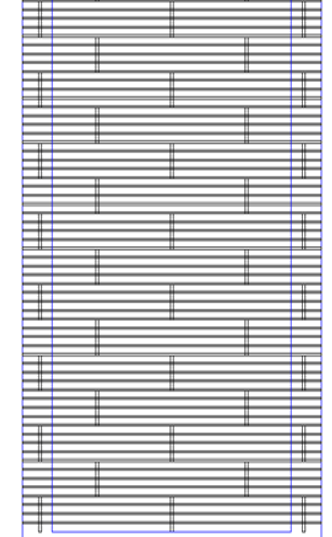
\includegraphics[angle=90,origin=c,width=3.6in]{figures/Collimator_Schema.png}

    \caption{The \acrshort{MSS} collimator design schematic show horizontal slits with vertical slats. Figure from \cite{8069508}} \label{fig:MSSColl}
%\vspace{-0.2cm}
\end{figure}

\begin{figure}[!t]
%\vspace{-0.2cm}
\centering
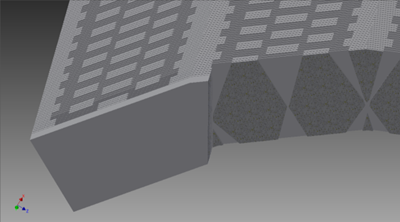
\includegraphics[width=3.6in]{figures/collimator.png}

    \caption{The cross section of the \acrshort{MSS} shows the slits embedded within the slats} \label{fig:MSSslit}
%\vspace{-0.2cm}
\end{figure}


To maintain \acrshort{MR} compatibility, tungsten is used in place of lead in this collimator. The collimator is composed of 6000 individual tungsten pieces, each electrically insulated. This design was chosen to prevent the induction of eddy currents within the metal \cite{7286864}. A continuous loop of metal can induce Eddy currents which in turn will induce an opposing force against the magnetic field. The series of slits run along the length of the collimator in alternating pairs and triplets, these are labelled the `2 slits' and the `$1 + 2\frac{1}{2}$ slits'. The furthest edge `$2\frac{1}{2}$ slits'  combine with those of the neighbouring collimator to cover a wider angular range across the ring. 
\paragraph{}
The \acrshort{FOV} covered by the slits in the trans-axial plane is 20 cm. The large \acrshort{FOV} is a result of the radially position slits and fanned out individual slits. The small system design leads to minification of the object in the the trans-axial plane, within the \acrshort{FOV}.The series of parallel slats running perpendicularly along the length of the slits define the resolution in the axial direction. The axial \acrshort{FOV} is 9 cm and induces no minification in this direction. Together the slits and slats define a cylindrical \acrshort{FOV}. The design is expected to give a resolution of 8 - 10 mm within the \acrshort{FOV}. 
\paragraph{}
 The use of the MSS collimator requires the implementation of a specific calibration procedure, which was established on a single detector system \cite{8340862}, and initially tested on a semi-operational system \cite{inproceedings}. The experiments within this thesis involve the use and assessment of this calibration technique, later chapters will discuss the effectiveness of this procedure.

\section{Current Work}
The \acrshort{INSERT} design has been established in a pre-clinical and clinical system. The pre-clinical system has been tested as a proof of concept and has been successfully implemented within a clinical \acrshort{MRI} scanner \cite{Carminati2018ExperimentalInsert}. The clinical system has undergone electrical testing and characterisation \cite{8432104}, but has not yet been implemented in an \acrshort{MRI} or evaluated for imaging capabilities. The work outlined in this thesis demonstrates the imaging potential of the stand alone \acrshort{SPECT} system and introduces a number of protocols and techniques which set out to ready the system for a complete integration within a clinical \acrshort{MRI}. The end goal of this research is to establish the first simultaneous acquisitions of \acrshort{SPECT/MRI} and carry out the first in man studies of this novel imaging technology. 

\begin{figure}[!t]
%\vspace{-0.2cm}
\centering
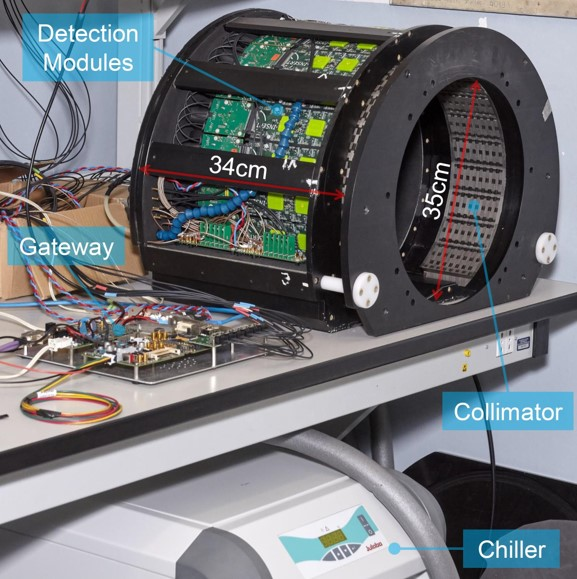
\includegraphics[width=3.6in]{figures/insert_system.jpg}

    \caption{The INSERT system complete with cooling system and control gateway.} \label{fig:CompINSERT}
%\vspace{-0.2cm}
\end{figure}